\subsection{KeyStone Federation}

\subsubsection{Federation简介}
KeyStone Federation实质上是不同的keystone之间的互信,因此,需要多个keystone实例。
Keystone Federation的现象就是,用户A在keystone1中存在,在keystone2中不存在,但是,
却依然能够通过keystone2的认证,并且访问keystone2所管理的服务。其工作的大致流程如
图 \colorunderlineref{fig:k2k_auth}

\begin{figure}[H]
  \centering
  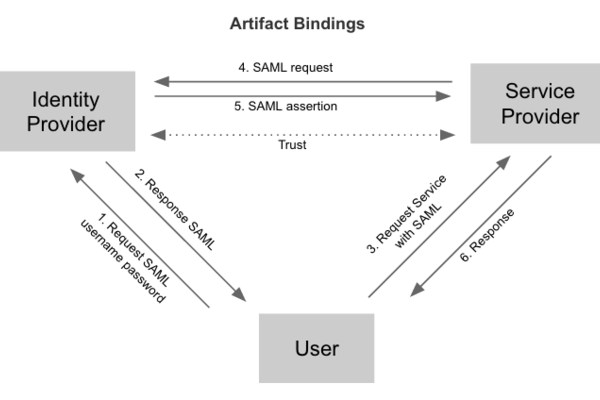
\includegraphics[width=\linewidth]{k2k_auth.png}
  \caption{Federation 流程\protect\footnotemark}
  \label{fig:k2k_auth}
\end{figure}
\footnotetext{来源:\url{http://wsfdl.com/openstack/2016/01/14/Keystone-Federation-Identity-with-SAML2.html}}

其中,keystone1就是认证提供者-Identity Provider(IdP),keystone2就是服务提供者-
Service Provider(SP)。

\subsubsection{Federation环境}
IdP:172.16.1.63

SP: 172.16.1.64

操作系统:Redhat 7

KeyStone版本:Mitaka

\subsubsection{IdP设置}

\begin{code-block}{bash}
yum install xmlsec1-openssl python-pysaml2 xmlsec1 shibboleth -y
export MY_IP=`ifconfig eth0 | grep -w inet | awk '{print $2}'`
openstack-config --set /etc/keystone/keystone.conf saml \
    certfile /etc/keystone/ssl/certs/ca.pem
openstack-config --set /etc/keystone/keystone.conf saml \
    keyfile /etc/keystone/ssl/private/cakey.pem
openstack-config --set /etc/keystone/keystone.conf saml \
    idp_entity_id http://$MY_IP:5000/v3/OS-FEDERATION/saml2/idp
openstack-config --set /etc/keystone/keystone.conf saml \
    idp_sso_endpoint http://$MY_IP:5000/v3/OS-FEDERATION/saml2/sso
openstack-config --set /etc/keystone/keystone.conf saml \
    idp_metadata_path /etc/keystone/keystone_idp_metadata.xml

keystone-manage saml_idp_metadata > /etc/keystone/keystone_idp_metadata.xml

chown -R keystone:keystone /etc/keystone
systemctl restart httpd

openstack project create --domain default --description "Demo Project" demo
openstack user create --domain default --project demo --project-domain default \
    --password demo demo
openstack role add --project demo --user demo --project-domain default \
    --user-domain default member

openstack service provider create keystone-sp --auth-url \
    http://172.16.1.64:5000/v3/OS-FEDERATION/identity_providers/keystone-idp/protocols/saml2/auth \
    --service-provider-url http://172.16.1.64:5000/Shibboleth.sso/SAML2/ECP
\end{code-block}

\subsubsection{SP设置}

\begin{code-block}{bash}
yum install xmlsec1-openssl python-pysaml2 xmlsec1 shibboleth -y
openstack-config --set /etc/keystone/keystone.conf auth \
    methods external,password,token,oauth1,saml2
openstack-config --set /etc/keystone/keystone.conf auth \
    saml2 keystone.auth.plugins.mapped.Mapped
\end{code-block}

修改/etc/shibboleth/attribute-map.xml为如下内容:
\begin{code-block}{xml}
<Attributes xmlns="urn:mace:shibboleth:2.0:attribute-map"
    xmlns:xsi="http://www.w3.org/2001/XMLSchema-instance">

    <Attribute name="urn:mace:dir:attribute-def:eduPersonPrincipalName" id="eppn">
        <AttributeDecoder xsi:type="ScopedAttributeDecoder"/>
    </Attribute>
    <Attribute name="urn:oid:1.3.6.1.4.1.5923.1.1.1.6" id="eppn">
        <AttributeDecoder xsi:type="ScopedAttributeDecoder"/>
    </Attribute>

    <Attribute name="urn:mace:dir:attribute-def:eduPersonScopedAffiliation" id="affiliation">
        <AttributeDecoder xsi:type="ScopedAttributeDecoder" caseSensitive="false"/>
    </Attribute>
    <Attribute name="urn:oid:1.3.6.1.4.1.5923.1.1.1.9" id="affiliation">
        <AttributeDecoder xsi:type="ScopedAttributeDecoder" caseSensitive="false"/>
    </Attribute>

    <Attribute name="urn:mace:dir:attribute-def:eduPersonAffiliation" id="unscoped-affiliation">
        <AttributeDecoder xsi:type="StringAttributeDecoder" caseSensitive="false"/>
    </Attribute>
    <Attribute name="urn:oid:1.3.6.1.4.1.5923.1.1.1.1" id="unscoped-affiliation">
        <AttributeDecoder xsi:type="StringAttributeDecoder" caseSensitive="false"/>
    </Attribute>

    <Attribute name="urn:mace:dir:attribute-def:eduPersonEntitlement" id="entitlement"/>
    <Attribute name="urn:oid:1.3.6.1.4.1.5923.1.1.1.7" id="entitlement"/>

    <Attribute name="openstack_user" id="openstack_user"/>
    <Attribute name="openstack_roles" id="openstack_roles"/>
    <Attribute name="openstack_project" id="openstack_project"/>
    <Attribute name="openstack_user_domain" id="openstack_user_domain"/>
    <Attribute name="openstack_project_domain" id="openstack_project_domain"/>

    <Attribute name="urn:mace:dir:attribute-def:eduPersonTargetedID" id="targeted-id">
        <AttributeDecoder xsi:type="ScopedAttributeDecoder"/>
    </Attribute>

    <Attribute name="urn:oid:1.3.6.1.4.1.5923.1.1.1.10" id="persistent-id">
        <AttributeDecoder xsi:type="NameIDAttributeDecoder"
            formatter="$NameQualifier!$SPNameQualifier!$Name" defaultQualifiers="true"/>
    </Attribute>

    <Attribute name="urn:oasis:names:tc:SAML:2.0:nameid-format:persistent" id="persistent-id">
        <AttributeDecoder xsi:type="NameIDAttributeDecoder"
            formatter="$NameQualifier!$SPNameQualifier!$Name" defaultQualifiers="true"/>
    </Attribute>

</Attributes>
\end{code-block}

修改/etc/shibboleth/shibboleth2.xml为如下内容:
\begin{code-block}{xml}
<SPConfig xmlns="urn:mace:shibboleth:2.0:native:sp:config"
    xmlns:conf="urn:mace:shibboleth:2.0:native:sp:config"
    xmlns:saml="urn:oasis:names:tc:SAML:2.0:assertion"
    xmlns:samlp="urn:oasis:names:tc:SAML:2.0:protocol"
    xmlns:md="urn:oasis:names:tc:SAML:2.0:metadata"
    clockSkew="7200">

    <ApplicationDefaults entityID="http://172.16.1.64:5000/Shibboleth.sso/SAML2/ECP">

        <Sessions lifetime="28800" timeout="3600" relayState="ss:mem"
                  checkAddress="false" handlerSSL="false" cookieProps="http">

            <SSO entityID="http://172.16.1.63:5000/v3/OS-FEDERATION/saml2/idp2" ECP="true">
              SAML2 SAML1
            </SSO>

            <Logout>SAML2 Local</Logout>

            <Handler type="MetadataGenerator" Location="/Metadata" signing="false"/>

            <Handler type="Status" Location="/Status" acl="127.0.0.1 ::1"/>

            <Handler type="Session" Location="/Session" showAttributeValues="false"/>

            <Handler type="DiscoveryFeed" Location="/DiscoFeed"/>
        </Sessions>

        <Errors supportContact="wei.d.chen@intel.com"
            helpLocation="/about.html"
            styleSheet="/shibboleth-sp/main.css"/>

        <MetadataProvider type="XML" uri="http://172.16.1.63:5000/v3/OS-FEDERATION/saml2/metadata"
              reloadInterval="7200">
        </MetadataProvider>

        <AttributeExtractor type="XML" validate="true" reloadChanges="false" path="attribute-map.xml"/>

        <AttributeResolver type="Query" subjectMatch="true"/>

        <AttributeFilter type="XML" validate="true" path="attribute-policy.xml"/>

        <CredentialResolver type="File" key="sp-key.pem" certificate="sp-cert.pem"/>

        <ApplicationOverride id="keystone-idp" entityID="http://172.16.1.64:5000/Shibboleth.sso/SAML2/ECP">
           <Sessions lifetime="28800" timeout="3600" checkAddress="false"
           relayState="ss:mem" handlerSSL="false">

            <SSO entityID="http://172.16.1.63:5000/v3/OS-FEDERATION/saml2/idp" ECP="true">
                SAML2 SAML1
            </SSO>

            <Logout>SAML2 Local</Logout>
           </Sessions>

           <MetadataProvider type="XML" uri="http://172.16.1.63:5000/v3/OS-FEDERATION/saml2/metadata"
             reloadInterval="180000" />

        </ApplicationOverride>
    </ApplicationDefaults>

    <SecurityPolicyProvider type="XML" validate="true" path="security-policy.xml"/>

    <ProtocolProvider type="XML" validate="true" reloadChanges="false" path="protocols.xml"/>

</SPConfig>
\end{code-block}

由于SP端需要一些特殊的设置,因此,不能使用原来的http conf文件来部署keystone,需要做如下的更改:
\begin{code-block}{bash}
cat >/etc/httpd/conf.d/wsgi-keystone.conf<<EOF
Listen 5000
Listen 35357

<VirtualHost *:5000>
    WSGIDaemonProcess keystone-public processes=5 threads=1 user=keystone group=keystone display-name=%{GROUP}
    WSGIProcessGroup keystone-public
    WSGIScriptAlias / /usr/bin/keystone-wsgi-public
    WSGIScriptAliasMatch ^(/v3/OS-FEDERATION/identity_providers/.*?/protocols/.*?/auth)$ /var/www/keystone/main/$1
    WSGIApplicationGroup %{GLOBAL}
    SetEnv Shib-Identity-Provider http://172.16.1.63:5000/v3/OS-FEDERATION/saml2/idp
    WSGIPassAuthorization On
    ErrorLogFormat "%{cu}t %M"
    ErrorLog /var/log/httpd/keystone-error.log
    CustomLog /var/log/httpd/keystone-access.log combined

    <Directory /usr/bin>
        Require all granted
    </Directory>
</VirtualHost>

<VirtualHost *:35357>
    WSGIDaemonProcess keystone-admin processes=5 threads=1 user=keystone group=keystone display-name=%{GROUP}
    WSGIProcessGroup keystone-admin
    WSGIScriptAlias / /usr/bin/keystone-wsgi-admin
    WSGIScriptAliasMatch ^(/v3/OS-FEDERATION/identity_providers/.*?/protocols/.*?/auth)$ /var/www/keystone/admin/$1
    WSGIApplicationGroup %{GLOBAL}
    SetEnv Shib-Identity-Provider http://172.16.1.63:35357/v3/OS-FEDERATION/saml2/idp
    WSGIPassAuthorization On
    ErrorLogFormat "%{cu}t %M"
    ErrorLog /var/log/httpd/keystone-error.log
    CustomLog /var/log/httpd/keystone-access.log combined

    <Directory /usr/bin>
        Require all granted
    </Directory>
</VirtualHost>

<Location /Shibboleth.sso>
    SetHandler shib
</Location>

<LocationMatch /v3/OS-FEDERATION/identity_providers/.*?/protocols/saml2/auth>
    ShibRequestSetting requireSession 1
    AuthType shibboleth
    ShibExportAssertion Off
    Require valid-user
</LocationMatch>
EOF
\end{code-block}

\begin{code-block}{bash}
mkdir -p /var/www/keystone
cp /usr/share/keystone/keystone.wsgi /var/www/keystone/admin
cp /usr/share/keystone/keystone.wsgi /var/www/keystone/main
chown -R keystone:keystone /var/www/keystone /etc/keystone
chmod 755 /var/www/keystone/*

/etc/shibboleth/keygen.sh  -f  -o /etc/shibboleth

systemctl restart httpd
systemctl enable shibd;systemctl start shibd
\end{code-block}

设置federation的映射组和domain等等关系
\begin{code-block}{bash}
openstack domain create federate_domain
openstack project create --domain federate_domain federate_project
openstack group create --domain federate_domain federate_group
openstack role add --project federate_project --group federate_group \
    --project-domain federate_domain --group-domain federate_domain member
\end{code-block}

添加IdP
\begin{code-block}{bash}
openstack identity provider create keystone-idp --remote-id http://172.16.1.63:5000/v3/OS-FEDERATION/saml2/idp
\end{code-block}

创建mapping映射规则
\begin{code-block}{bash}
cat > /root/mapping.json<<EOF
[
    {
        "local": [
            {
                "user": {
                    "name": "{0}"
                },
                "group": {
                    "name": "federate_group",
                    "domain": {
                        "name": "federate_domain"
                    }
                }
            }
        ],
        "remote": [
            {
                "type": "openstack_user"
            },
            {
                "type": "openstack_user_domain"
            },
            {
                "type": "openstack_project"
            },
            {
                "type": "openstack_project_domain"
            },
            {
                "type": "openstack_roles"
            }
        ]
    }
]
EOF
openstack mapping create k2k --rules /root/mapping.json
\end{code-block}

关联IdP和mapping映射规则
\begin{code-block}{bash}
openstack federation protocol create saml2 --identity-provider keystone-idp --mapping k2k
\end{code-block}

\subsubsection{校验Federation}
\begin{code-block}{python}
import json
import os

import requests

from keystoneclient import session as ksc_session
from keystoneclient.auth.identity import v3
from keystoneclient.v3 import client as keystone_v3


class K2KClient(object):
    def __init__(self):
        # auth_url一定是IdP的url,username,password,domain_main
        # 都是IdP端的,不是SP端的
        self.sp_id = 'keystone-sp'
        self.auth_url = 'http://172.16.1.63:35357/v3'
        self.username = 'admin'
        self.password = 'admin'
        self.domain_name = 'default'

    def v3_authenticate(self):
        auth = v3.Password(auth_url=self.auth_url,
                           username=self.username,
                           password=self.password,
                           user_domain_name=self.domain_name)
        self.session = ksc_session.Session(auth=auth, verify=False)
        self.session.auth.get_auth_ref(self.session)
        self.token = self.session.auth.get_token(self.session)

    def _generate_token_json(self):
        return {
            "auth": {
                "identity": {
                    "methods": [
                        "token"
                    ],
                    "token": {
                        "id": self.token
                    }
                },
                "scope": {
                    "service_provider": {
                        "id": self.sp_id
                    }
                }
            }
        }

    def _check_response(self, response):
        if not response.ok:
            raise Exception("Something went wrong, %s" % response.__dict__)

    def get_saml2_ecp_assertion(self):
        token = json.dumps(self._generate_token_json())
        url = self.auth_url + '/auth/OS-FEDERATION/saml2/ecp'
        r = self.session.post(url=url, data=token, verify=False)
        self._check_response(r)
        self.assertion = str(r.text)

    def _get_sp(self):
        url = self.auth_url + '/OS-FEDERATION/service_providers/' + self.sp_id
        r = self.session.get(url=url, verify=False)
        self._check_response(r)
        sp = json.loads(r.text)[u'service_provider']
        return sp

    def _handle_http_302_ecp_redirect(self, response, location, **kwargs):
        return self.session.get(location, authenticated=False, **kwargs)

    def exchange_assertion(self):
        """Send assertion to a Keystone SP and get token."""
        sp = self._get_sp()

        r = self.session.post(
            sp[u'sp_url'],
            headers={'Content-Type': 'application/vnd.paos+xml'},
            data=self.assertion,
            authenticated=False,
            redirect=False)

        self._check_response(r)

        r = self._handle_http_302_ecp_redirect(r, sp[u'auth_url'],
                                               headers={'Content-Type':
                                               'application/vnd.paos+xml'})
        self.fed_token_id = r.headers['X-Subject-Token']
        self.fed_token = r.text

    def list_federated_projects(self):
        url = 'http://172.16.1.64:5000/v3/OS-FEDERATION/projects'
        headers = {'X-Auth-Token': self.fed_token_id}
        r = requests.get(url=url, headers=headers)
        self._check_response(r)
        return json.loads(str(r.text))

    def _get_scoped_token_json(self, project_id):
        return {
            "auth": {
                "identity": {
                    "methods": [
                        "token"
                    ],
                    "token": {
                        "id": self.fed_token_id
                    }
                },
                "scope": {
                    "project": {
                        "id": project_id
                    }
                }
            }
        }

    def scope_token(self, project_id):
        # project_id can be select from the list in the previous step
        token = json.dumps(self._get_scoped_token_json(project_id))
        url = 'http://172.16.1.64:5000/v3/auth/tokens'
        headers = {'X-Auth-Token': self.fed_token_id,
                   'Content-Type': 'application/json'}
        r = requests.post(url=url, headers=headers, data=token,
                          verify=False)
        self._check_response(r)
        self.scoped_token_id = r.headers['X-Subject-Token']
        self.scoped_token = str(r.text)

    def get_images(self):
        # 如果SP端配置了glance,可以用这个方法来测试federation的真正使用。
        url = 'http://172.16.1.64:9292/v2/images?limit=20&sort_key=name&sort_dir=asc'
        headers = {'X-Auth-Token': self.fed_token_id,
                   'Content-Type': 'application/json'}
        r = requests.get(url=url, headers=headers)
        print r.text


def main():
    client = K2KClient()
    client.v3_authenticate()
    client.get_saml2_ecp_assertion()
    client.exchange_assertion()
    print('Unscoped token id: %s' % client.fed_token_id)

    # If you want to get a scope token, please ensure federated_user has a project
    # and uncommen below codes.
    projects = client.list_federated_projects()
    print('Federated projects: %s' % projects['projects'])
    project_id = projects['projects'][0]['id']
    project_name = projects['projects'][0]['name']
    client.scope_token(project_id)
    print('Scoped token of ' + project_name + ' : ' + client.scoped_token_id)
    print client.scoped_token
    #client.get_images()


if __name__ == "__main__":
    main()
\end{code-block}

将以上的内容名为为k2k.py文件,然后执行,如果出现如图 \colorunderlineref{fig:k2k_result}的输出,就证明keystone federation
配置成功了。
\begin{figure}[H]
  \centering
  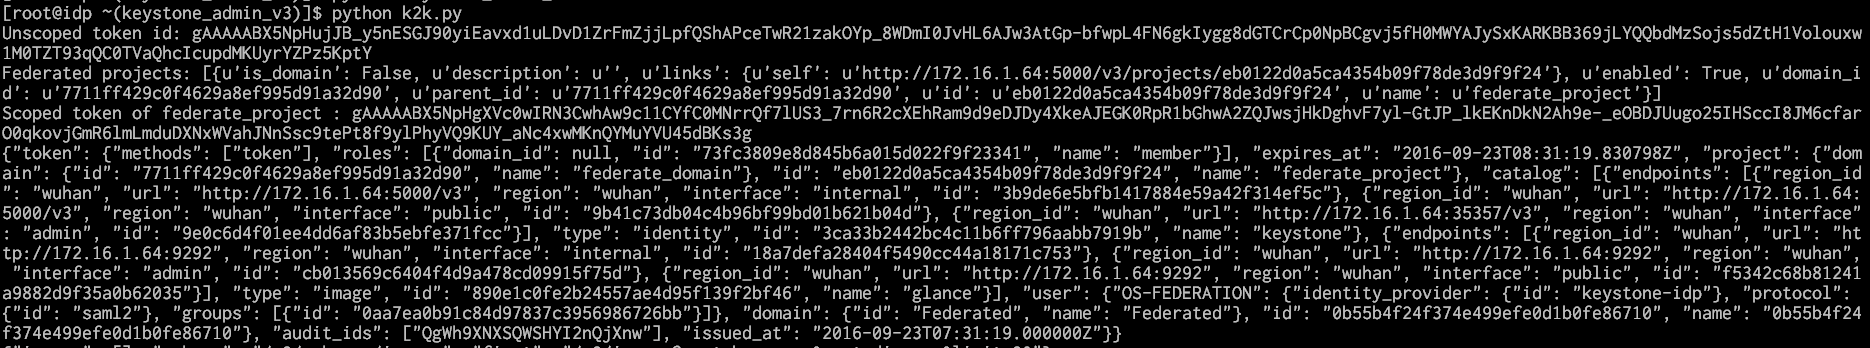
\includegraphics[width=\linewidth]{k2k_result.png}
  \caption{Federation 测试}
  \label{fig:k2k_result}
\end{figure}

从Mitaka开始,oepnstack官方提供了k2k的client支持。
\begin{code-block}{python}
from keystoneauth1 import session
from keystoneauth1.identity import v3
from keystoneauth1.identity.v3 import k2k

from glanceclient import Client
from cinderclient.v2 import client as cinder
from novaclient.v2 import client as nova

auth = v3.Password(auth_url='http://172.16.1.63:5000/v3',
                   username='admin',
                   password='admin',
                   user_domain_name='default')
password_session = session.Session(auth=auth, verify=False)

password_session.auth.get_auth_ref(password_session)

token_auth = v3.Token(auth_url=auth_url, token=unscoped_idp_token,
                      project_name='admin',
                      project_domain_name='default')
token_session = session.Session(auth=token_auth, verify=False)
try:
    token_session.auth.get_auth_ref(token_session)
except exceptions.http.Unauthorized as exc:
    raise exc

k2ksession = k2k.Keystone2Keystone(token_session.auth,
    'keystone-sp', project_name='federate_project',
    project_domain_name='federate_domain')

access = k2ksession.get_auth_ref(token_session)

scoped_token_id = access._auth_token

image_url = k2ksession.get_endpoint(token_session,
                                    service_type='image')

glance = Client('2', endpoint=image_url, token=scoped_token_id)
images = glance.images.list()
for image in images:
    print image

cinder_client = cinder.Client(session=token_session, auth=k2ksession)
volumes = cinder_client.volumes.list()
for vol in volumes:
    print vol.to_dict()

nova_client = nova.Client(session=token_session, auth=k2ksession)
servers = nova_client.servers.list()
for server in servers:
    print server.to_dict()
\end{code-block}

\subsubsection{KeyStone Federation工作流程}
Keystone Federation的工作与单独的keystone的工作流程区别比较大,主要分为如下几个步骤:
\begin{enumerate}
  \item 获取idp的unscope token
  \item 通过unscope token获取idp端的scope token
  \item 通过scope token获取saml断言
  \item 在sp端校验saml断言,并返回cookie
  \item 使用cookie获取sp端的unscope token
  \item 通过sp端的unscope token获取可用的scope token
  \item 使用sp端的scope token访问sp端的服务,获取资源
\end{enumerate}

\paragraph{IdP用户获取unscoped token}
\begin{code-block}{bash}
cat >unscope.json<<EOF
{
    "auth": {
        "identity": {
            "methods": [
                "password"
            ],
            "password": {
                "user": {
                    "domain": {
                        "name": "default"
                    },
                    "name": "demo",
                    "password": "demo"
                }
            }
        }
    }
}
EOF
export UNSCOPE_TOKEN=`curl -i -X POST http://172.16.1.63:5000/v3/auth/tokens \
    -H "Content-Type: application/json" \
    -d @unscope.json | grep X-Subject-Token | awk '{print $2}' | strings`
\end{code-block}

\paragraph{IdP用户获取scoped token}
\begin{code-block}{bash}
cat >scope.json<<EOF
{
    "auth": {
        "identity": {
            "methods": [
                "token"
            ],
            "token": {
                "id": "$UNSCOPE_TOKEN"
            }
        },
        "scope": {
            "project": {
                "name": "demo",
                "domain": {
                    "name": "default"
                }
            }
        }
    }
}
EOF
export SCOPE_TOKEN=`curl -i -X POST http://172.16.1.63:5000/v3/auth/tokens \
    -H "Content-Type: application/json" \
    -d @scope.json | grep X-Subject-Token | awk '{print $2}' | strings`
\end{code-block}

\paragraph{获取saml断言}
\begin{code-block}{bash}
cat >saml.json<<EOF
{
    "auth": {
        "identity": {
            "methods": [
                "token"
            ],
            "token": {
                "id": "$SCOPE_TOKEN"
            }
        },
        "scope": {
            "service_provider": {
                "id": "keystone-sp"
            }
        }
    }
}
EOF
curl -X POST http://172.16.1.63:5000/v3/auth/OS-FEDERATION/saml2/ecp \
    -H "Content-Type: application/json" \
    -d @saml.json > assertion
\end{code-block}

\paragraph{SP端校验saml断言}
\begin{code-block}{bash}
export SAML_COOKIE=`curl -X POST -i http://172.16.1.64:5000/Shibboleth.sso/SAML2/ECP \
    -H "Content-Type: application/vnd.paos+xml" \
    -d @assertion | grep Set-Cookie | awk '{print $2}'`
\end{code-block}

\paragraph{SP端获取unscope token}
\begin{code-block}{bash}
export SP_UNSCOPE_TOKEN=`curl -i -X GET \
    http://172.16.1.64:5000/v3/OS-FEDERATION/identity_providers/keystone-idp/protocols/saml2/auth \
    -H "Content-Type: application/vnd.paos+xml" \
    -b $SAML_COOKIE | grep X-Subject-Token | awk '{print $2}' | strings`
\end{code-block}

\colorblock{特别需要说明的是,IdP和SP端的用户映射就是在这一个步骤当中完成的。}

\paragraph{SP端获取scope token}
\begin{code-block}{bash}
cat >spscope.json<<EOF
{
    "auth": {
        "identity": {
            "methods": [
                "token"
            ],
            "token": {
                "id": "$SP_UNSCOPE_TOKEN"
            }
        },
        "scope": {
            "project": {
                "name": "demo",
                "domain": {
                    "name": "default"
                }
            }
        }
    }
}
EOF
export SP_SCOPE_TOKEN=`curl -i -X POST http://172.16.1.64:5000/v3/auth/tokens \
    -H "Content-Type: application/json" \
    -d @spscope.json | grep X-Subject-Token | awk '{print $2}' | strings`
\end{code-block}

经过以上几个步骤之后,使用SP\_SCOPE\_TOKEN就可以访问SP端提供的所有服务了。

\subsubsection{参考文献}
\url{http://blog.rodrigods.com/it-is-time-to-play-with-keystone-to-keystone-federation-in-kilo/}

\url{http://wsfdl.com/openstack/2016/01/14/Keystone-Federation-Identity-with-SAML2.html}

\url{https://wiki.shibboleth.net/confluence/display/SHIB2/Configuration}

\url{http://blog.csdn.net/chenwei8280/article/details/49560963}
